\section{C3: when does a learned KKL observer beat a model-based filter?}\label{sec:c3}

\paragraph{Question and rules.} The best KKL observer (HyperKKL, its dense ablation or latent injection, as pre-registered) is compared with the best of eight model-based filters, paired on the same episodes, on \tier{id} and \tier{sequence\_ood}; ``learned wins'' in a scenario needs a CI excluding 0 on $\ge4/6$ dev plants on both tiers. The filters hold the modeller's model; the learned observers are trained on labelled data from the real plant. Absolute NRMSE accompanies every change; a filter above \emph{climatology} is FAILED, and changes are quoted against the best \emph{working} filter with the number of failed filters. Scenarios: exact model under fifteen stress conditions (\node{C3-faults}, descriptive), coloured Student-$t$ noise in training and deployment (\node{C3-noise-ct}), parameter mismatch at four levels (\node{C3-mismatch10/20/30/50}; hypothesis: the crossover sits between 10\% and 30\%), a missing physical term (\node{C3-partial}, descriptive, against the relative model error), and the realistic deployment (\node{C3-realistic}).

\begin{figure}[t]
\centering
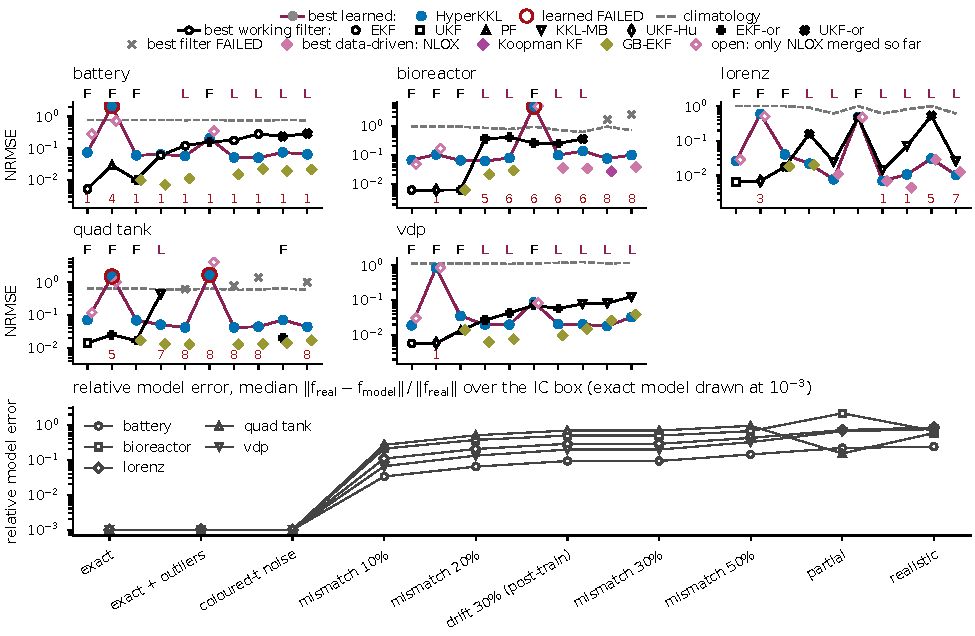
\includegraphics[width=0.68\textwidth, trim=0 140 0 0, clip]{fig3_c3_crossover.pdf}
\caption{C3 on the dev plants, \tier{sequence\_ood}, NRMSE on a log axis: best learned observer (coloured by method) against the best working filter (black) and climatology (dashed), per scenario ordered by the median relative model error over plants (the model-error panel of the generated figure is omitted here; the values are in Table~\ref{tab:systems} and in Figure~\ref{fig:c3id}). Top marks: L = learned beats the best working filter (paired 95\% CI), F = filter wins; red numbers = filters above climatology. Red-ringed markers: the best \emph{learned} observer is itself above climatology. Grey crosses: the best filter is FAILED and there is no working filter. The \tier{id} version and the held-out plants are in Appendix~\ref{app:tables}.}
\label{fig:c3}
\end{figure}

\paragraph{Exact model: the filters win everywhere.} In none of the fifteen stress conditions does the learned side reach the learned-wins regime (\node{C3-faults}: \CthreeFaultsRegimes), against nominal and robust/oracle filters alike (Tables~\ref{tab:c3} and \ref{tab:decisions}). Under coloured heavy-tailed noise in training and deployment the learned observers beat the best filter on \CthreeNoiseCtSeqVsWorking\ plants (\node{C3-noise-ct}: \OutcomeCThreeNoiseCt). Two exact-model failures of the learned observers: under 2\% gross sensor outliers the best learned observer is itself above climatology on \sys{battery}, \sys{duffing} and \sys{quad\_tank}, while the Huber and oracle filters keep their clean accuracy (Table~\ref{tab:c3full}); and after a 30\% plant drift that occurs \emph{after} training, it is above climatology on \sys{bioreactor} and \sys{quad\_tank}. These limits of the method as trained here (nominal sensor, no robust loss, no adaptation) are consistent with the theory: the fault's effect is multiplied by a decoder slope in the hundreds (Corollary~\ref{cor:m3-faults}, Remark~\ref{rem:m3-cert}), and on linear plants a Kalman filter beats any KKL observer with outliers too (Remark~\ref{rem:m3-kf}).

% generated by analysis/paper_results.py -- do not edit by hand
% requires \usepackage{booktabs,longtable,array}
\begin{table}[t]
\centering
\scriptsize
\setlength{\tabcolsep}{2pt}
\caption{When does a learned KKL observer win (C3)? sequence OOD, dev plants: number of plants on which HyperKKL ($r=4$, the single learned method) beats the comparator (paired 95\% CI excludes 0). Per-plant numbers: Table~\ref{tab:c3full}.}
\label{tab:c3}
\begin{tabular}{@{}lrrrrrrrr@{}}
\toprule
 & & \multicolumn{5}{c}{(a) vs model-based filters} & \multicolumn{2}{c}{(b) vs data-driven} \\
\cmidrule(lr){3-7}\cmidrule(l){8-9}
scenario & model err. & best filter & working & nominal & rob./orac. & failed & best data-driven & NLOX \\
\midrule
exact & 0.00 & 0/5 (5L) & 0/5 (5L) & 0/5 (5L) & 0/5 (5L) & 1/40 & pend.\ 0/25 & 3/5 \\
exact+outliers & 0.00 & 0/5 (5L) & 0/5 (5L) & 0/5 (5L) & 0/5 (5L) & 14/40 & pend.\ 0/25 & 1/5 (3L) \\
colored\_t & 0.00 & 0/5 (5L) & 0/5 (5L) & 0/5 (5L) & 0/5 (5L) & 1/40 & 0/5 (5L) & 4/5 \\
mismatch10 & 0.11 & 4/5 & 4/5 & 4/5 & 4/5 & 13/40 & 0/5 (4L) & 3/5 \\
mismatch20 & 0.20 & 5/5 & 4/4$^*$ & 5/5 & 5/5 & 15/40 & 1/5 (4L) & 4/5 (1L) \\
drift30 (post-train) & 0.29 & 0/5 (4L) & 0/4 (4L)$^*$ & 2/5 (2L) & 1/5 (4L) & 15/40 & pend.\ 0/25 & 2/5 (1L) \\
mismatch30 & 0.29 & 5/5 & 4/4$^*$ & 5/5 & 5/5 & 16/40 & 0/5 (3L) & 3/5 \\
mismatch50 & 0.42 & 5/5 & 4/4$^*$ & 5/5 & 5/5 & 16/40 & 0/5 (3L) & 3/5 \\
partial & 0.66 & 4/5 (1L) & 3/4 (1L)$^*$ & 4/5 (1L) & 4/5 (1L) & 14/40 & 1/5 (3L) & 3/5 (1L) \\
realistic & 0.68 & 5/5 & 3/3$^*$ & 5/5 & 5/5 & 24/40 & 2/5 (3L) & 4/5 (1L) \\
\bottomrule
\end{tabular}
\par\smallskip\begin{minipage}{\linewidth}\scriptsize ($k$L): the comparator is significantly better on $k$ plants. (a) Model-based filters: EKF, UKF, PF, KKL-MB and their Huber and oracle variants. A filter is FAILED when its NRMSE exceeds climatology (the constant mean-state predictor); `working' = the best filter that did not fail ($^*$: no filter works on some plants). (b) Data-driven baselines trained on the same real-plant data: NLOX, Koopman KF (incl.\ bilinear), grey-box EKF/UKF/EKF-oracle; `pend.\ $m/N$' = merged in $m$ of $N$ runs. Model error: median over dev plants.\end{minipage}
\end{table}


\paragraph{Wrong model: the learned observers win at every level tested.} With the real plant's parameters off nominal, the learned side beats the best filter on \CthreeMismatchTenIdVsWorking\ (\tier{id}) and \CthreeMismatchTenSeqVsWorking\ (\tier{sequence\_ood}) plants at 10\% (\OutcomeCThreeMismatchTen), \CthreeMismatchTwentyIdVsWorking\ and \CthreeMismatchTwentySeqVsWorking\ at 20\% (\OutcomeCThreeMismatchTwenty), \CthreeMismatchThirtyIdVsWorking\ and \CthreeMismatchThirtySeqVsWorking\ at 30\% (\OutcomeCThreeMismatchThirty), \CthreeMismatchFiftyIdVsWorking\ and \CthreeMismatchFiftySeqVsWorking\ at 50\% (\OutcomeCThreeMismatchFifty); the same counts hold against the robust/oracle filters, which are given the model-error rate in $Q$. The pre-registered crossover hypothesis therefore \FAIL s (\node{C3-mismatch (crossover)}: \OutcomeCThreeMismatchCrossover): the first winning level is the smallest one tested, and the crossing, if there is one, lies below 10\%. The exception at every level is \sys{duffing}, whose 30\% parameter error moves $f$ by only \ModelErrDuffingMismatchThirty\ in relative terms (Table~\ref{tab:systems}) and whose best filter stays several times better (\CthreeMismatchThirtySeqDuffingBestWorking\ against \CthreeMismatchThirtySeqDuffingBestLearned\ at 30\%); \sys{battery} at 10\% is the other non-win on \tier{sequence\_ood} (\CthreeMismatchTenSeqBatteryVsWorking, n.s.). With one physical term missing (\node{C3-partial}: \OutcomeCThreePartial), the learned side wins on \CthreePartialIdVsWorking\ and \CthreePartialSeqVsWorking\ plants; the exception is \sys{quad\_tank}, where linearising the orifice law moves $f$ by \ModelErrQuadTankPartial\ and the oracle EKF wins (\CthreePartialSeqQuadTankBestWorking\ against \CthreePartialSeqQuadTankBestLearned), whereas \sys{bioreactor} (relative model error \ModelErrBioreactorPartial), \sys{lorenz} (\ModelErrLorenzPartial) and \sys{vdp} (\ModelErrVdpPartial) are won at every level and \sys{duffing} (\ModelErrDuffingPartial) is won here. The pattern hypothesised for this node (learned wins on \sys{bioreactor}/\sys{vdp}/\sys{lorenz}, filters on \sys{duffing}/\sys{quad\_tank}) holds on four of its five named plants (Table~\ref{tab:decisions}).

\paragraph{Realistic deployment.} With partial model, 30\% parameter error and coloured Student-$t$ noise at once, the learned observers win on \CthreeRealisticIdVsWorking\ (\tier{id}) and \CthreeRealisticSeqVsWorking\ (\tier{sequence\_ood}) plants against the best filter of any kind and against the best working filter (\node{C3-realistic}: \OutcomeCThreeRealistic). On \sys{bioreactor} and \sys{quad\_tank} all eight filters are above climatology (\CthreeRealisticSeqBioreactorFailedFilters, \CthreeRealisticSeqQuadTankFailedFilters), so no change is quoted: the learned observers reach \CthreeRealisticSeqBioreactorBestLearned\ and \CthreeRealisticSeqQuadTankBestLearned\ against climatology \CthreeRealisticSeqBioreactorClimatology\ and \CthreeRealisticSeqQuadTankClimatology. On \sys{lorenz} \CthreeRealisticSeqLorenzFailedFilters\ filters fail and the working one, \texttt{kkl\_mb}, is beaten by \CthreeRealisticSeqLorenzVsWorking; \sys{battery}, \sys{duffing} and \sys{vdp} by \CthreeRealisticSeqBatteryVsWorking, \CthreeRealisticSeqDuffingVsWorking\ and \CthreeRealisticSeqVdpVsWorking.

\paragraph{Reading the crossover.} Over the 36 model-wrong cells (six plants $\times$ mismatch 10--50\%, partial, realistic), every non-win sits at a small relative model error (\sys{duffing}, \sys{battery} at 10\%, \sys{quad\_tank} partial) and every plant with a large error is won at every level (Figure~\ref{fig:c3}, Table~\ref{tab:c3full}): the single crossing Proposition~\ref{prop:m3-mismatch} predicts, at a plant- and noise-dependent value (Appendix~\ref{sec:m3}).

\paragraph{Two findings, not one.} (a) \emph{Learning from real-plant data beats model-based filters once the model is wrong.} This is the robust finding: it holds against nominal, robust and oracle-tuned filters, at every mismatch level, under a missing term and in the realistic node, and it reverses whenever the model is exact. (b) \emph{Which learner wins is system-dependent and is not settled here.} Two further estimators trained on exactly the learned observers' data are implemented: \texttt{koopman\_kf} (EDMD with inputs on a thin-plate-RBF dictionary, then a Kalman filter on the lifted state) and \texttt{greybox\_ekf/ukf} (the modeller's model plus an MLP residual fitted to the one-step defect, inside the unchanged EKF/UKF). This comparison (b), best KKL observer against the best data-driven baseline (NLOX included), was added after review and is \emph{not} pre-registered; it is merged into the runs node by node (column (b) of Table~\ref{tab:c3}). Where it is complete enough to decide, \node{C3-partial}, the KKL observers do \emph{not} win: \OutcomeCThreePartialDataDriven\ (KKL beats the best data-driven baseline on \CthreePartialIdVsDataDriven\ plants on \tier{id} and \CthreePartialSeqVsDataDriven\ on \tier{sequence\_ood}): on \tier{sequence\_ood} the grey-box EKF/UKF is better on \sys{battery} (\CthreePartialSeqBatteryBestDataDriven\ against \CthreePartialSeqBatteryBestLearned) and \sys{duffing} (\CthreePartialSeqDuffingBestDataDriven\ vs \CthreePartialSeqDuffingBestLearned), the Koopman KF on \sys{bioreactor}, and the KKL observers are better on \sys{lorenz} (\CthreePartialSeqLorenzVsDataDriven\ vs NLOX) and \sys{vdp} (\CthreePartialSeqVdpVsDataDriven\ vs the grey-box EKF). For the mismatch, realistic and held-out nodes comparison (b) is \OutcomeCThreeRealisticDataDriven\ at the time of writing (merge counts in Table~\ref{tab:c3}). So \emph{no claim that the KKL observer is the best learner is made}.
% TODO (pending, 05:07 / 08:07 Dubai regeneration): once koopman_kf / greybox_* appear in
% paper/generated (tab2_c3*.tex, numbers.tex), replace the sentence above by the generated counts
% (learned KKL vs same-data baselines, paired CI) and update the abstract, Section 1 item 2 and
% Section 9 accordingly. Never state a winner that the generated tables do not show.
Nor does C3 establish that the partial model helps the learned observer: the pre-registered test of the phase-1 PDE term with the partial model against a model-free phase 1 \FAIL s (\node{C3-partial-modelfree}: \OutcomeCThreePartialModelfree; the differences are not significant at three seeds, including a large but non-significant one on \sys{bioreactor}), so no claim that the partial model helps is made. Whether the KKL observers' structural advantages (global convergence, no linearisation) show against the grey-box filters where they should, under a poor initial guess, outliers, higher noise, post-training drift and a sensor outage with partial knowledge, is the question of a further node, \node{C3-regimes} (pre-registered rule: a KKL-wins regime needs $\ge4/6$ dev plants per condition on \tier{sequence\_ood}), whose outcome is \textcolor{red}{\textbf{\OutcomeCThreeRegimes}} at the time of writing. The replication on the held-out plants (\node{TEST-C3}, the realistic scenario) is \OutcomeTESTCThree\ at the time of writing with \JobsTESTCThree\ jobs finished: the learned side wins on \sys{fhn} (\CthreeTESTCThreeSeqFhnVsWorking\ on \tier{sequence\_ood}) and \sys{highway\_traffic} (\CthreeTESTCThreeSeqHighwayTrafficVsWorking), the UKF wins on \sys{cartpole} (\CthreeTESTCThreeSeqCartpoleVsWorking) although its realistic model error (partial \ModelErrCartpolePartial, 30\% \ModelErrCartpoleMismatchThirty) is comparable to that of dev plants the learned side won; with half the plants finished, no reading of the held-out crossover is offered.
% TODO (pending results): TEST-C3 is refreshed by the 05:00 / 08:00 regeneration; re-read this
% paragraph and the abstract sentence on held-out C3 once the node is decided.
